 
\chapter{ Mediation Analysis: Natural Direct and Indirect Effects}
 \label{chapter::mediation}




With an intermediate variable $M$ between the treatment $Z$ and outcome $Y$,  the causal effects within principal strata defined by $U = \{  M(1), M(0) \}$ can assess the treatment effect heterogeneity across latent groups $U$. When $M$ is indeed on the causal pathway from $Z$ to $Y$, causal effects within some principal strata, $\tau(1,1)$ and $ \tau(0,0)$, can give information about the direct effect of $Z$ on $Y$. However, these direct effects are only for two latent groups. The causal effects within the other two principal strata, $\tau(1,0)$ and $ \tau(0,1)$, contain both direct and indirect effects. Fundamentally, principal stratification does not provide any information about the indirect effect of $Z$ on $Y$ through $M$ because it does not even assume that $M$ can be intervened. 



In the above discussion, I use the notions of ``direct effect'' and ``indirect effect'' in a casual way. When $M$ lies on the pathway from $Z$ to $Y$, researchers often want to assess the extent to which the effect of $Z$ on $Y$ is through $M$ and the extent to which the effect is through other pathways. This is called {\it mediation analysis}. It is the topic of this chapter. 



\section{Motivating Examples}





In mediation analysis, we have a treatment $Z$, an outcome $Y$, a mediator $M$, and some background covariates $X$. Figure \ref{fg::mediationDAG} illustrates their relationship. Below we give some concrete examples. 



\begin{figure}[ht]
\centering
$$
\begin{xy}
\xymatrix{
&& X \ar[dll] \ar[d] \ar[drr] \\
Z \ar[rr] \ar@/_1.5pc/[rrrr] & & M\ar[rr] & & Y}
\end{xy}
$$
\caption{Causal diagram for mediation analysis}\label{fg::mediationDAG}
\end{figure}


\begin{example}
\citet{Vanderweele::2012genetic} conducted mediation analysis to assess the extent to which the effect of variants on chromosome 15q25.1 on lung cancer is mediated through smoking and the extent to which it operates through other causal pathways\footnote{Recall Chapter \ref{chapter::evalue} for Fisher's hypothesis of a common genetic factor that affects the smoking behavior and lung cancer simultaneously.}. The exposure levels correspond to changes from 0 to 2 C alleles, smoking intensity is measured by the square root of cigarettes per day, and the outcome is the lung cancer indicator. \citet{Vanderweele::2012genetic}'s study contained many sociodemographic covariates.  %case-control
\end{example}



\begin{example}
\citet{rudolph2018causal} studied the causal mechanism from neighborhood poverty to adolescent substance use, mediated by the school and peer environment. They used data from the National Comorbidity Survey Replication Adolescent Supplement, a nationally representative survey of U.S. adolescents conducted during 2001--2004. The treatment is the binary indicator of neighborhood disadvantage, defined as living in the lowest tertile of neighborhood socioeconomic status based on data from the 2000 U.S. Census. 
Four binary mediators are measures of school and peer environments, and six binary outcomes are measures of substance use. 
Baseline covariates included the adolescent's sex, age, race, immigration generation, family income, etc.
\end{example}


\begin{example}\label{eg::mediation-jobs}
The \ri{mediation} package in \ri{R} contains a dataset called \ri{jobs}, which is from JOBS II, a randomized field experiment that investigates the efficacy of a job training intervention on unemployed workers. 
We used this dataset in Chapter \ref{sec::cace-application}. 
The program is designed to not only increase reemployment among the unemployed but also enhance the mental health of the job seekers. It is therefore of interest to assess the indirect effect of the intervention on mental health through job search efficacy and its direct effect acting through other pathways. We will revisit this example in Chapter \ref{section::BK-jobs} later. 
\end{example}



\section{Nested Potential Outcomes}


\subsection{Natural Direct and Indirect Effects}
Below we drop the index $i$ for unit $i$ and assume all random variables are IID draws from a superpopulation. For simplicity, we focus on a binary treatment $Z$. 

 
We first consider the hypothetical intervention on $z$ and define potential mediators and outcomes corresponding to the intervention on $z$:
$$
\{ M(z) , Y(z): z=0,1\}.
$$
We then consider hypothetical intervention on both $z$ and $m$ and define potential outcomes corresponding to the interventions on $z$ and $m$:
$$
\{ Y(z, m): z=0, 1; m \in \mathcal{M}  \},
$$
where $ \mathcal{M} $ contains all possible values of $m$. 
\citet{Robins::1992} and \citet{Pearl::2001} further consider the nested potential outcomes corresponding to intervention on $z$ and $m = M(z')  $:
$$
\{ Y(z, M_{z'}) : z = 0,1; z'=0,1   \}
$$
where I write $M(z')$ as $ M_{z'}$ to avoid excessive parentheses. The notation $Y(z, M_{z'})$ is the hypothetical outcome if the treatment were set at level $z$ and the mediator were set at its potential level $M(z')$ under treatment $z'$. Importantly, $z$ and $z'$ can be different.
With a binary treatment, we have four nested potential outcomes in total:
$$
\{ Y( 1, M_1),    Y( 1, M_0),  Y( 0, M_1),  Y( 0, M_0) \}.
$$
The nested potential outcome  $Y(1, M_1)$ is the hypothetical outcome if the treatment were set at $z=1$ and the mediator were set at what would happen under $z=1$. Similarly, $Y(0, M_0)$ is the outcome if the treatment were set at $z=0$ and the mediator were set at what would happen under $z=0$. It would be surprising if $Y(1, M_1) \neq  Y(1)$ or $Y(0, M_0) \neq  Y(0)$.
Therefore, we make the following composition assumption throughout this chapter.

\begin{assumption}
[composition]\label{assume::composition}
$Y(z, M_z) =   Y(z)$ for $z=0,1$. 
\end{assumption}


The composition assumption cannot be proved. It is indeed an assumption. Without causing philosophical debates, we can even define $Y(1)$ as  $Y(1, M_1)$, and define $ Y(0)$ as $Y(0, M_0) $.  Then by definition, Assumption \ref{assume::composition} holds. 



The nested potential outcome $Y(1,M_0)$ is the hypothetical outcome if the unit received treatment $1$ but its mediator were set at its natural value $M_0$ without the treatment. Similarly, $Y(0,M_1)$ is the hypothetical outcome if the unit received control $0$ but its mediator were set at its natural value $M_1$ under the treatment. They are two cross-world counterfactual terms and are useful for defining the direct and indirect effects. 


\begin{definition}
[total, direct and indirect effects]
\label{def::mediation}
Define the total effect of the treatment on the outcome as
$$
\tau = E\{ Y(1)  - Y(0) \}.
$$
Define the natural direct effect as
$$
\NDE = E\{  Y(1,M_0) - Y(0, M_0)  \}. 
$$
Define the natural indirect effect as 
$$
\NIE = E\{  Y(1, M_1) - Y(1, M_0) \} .
$$
\end{definition}


The total effect is the standard average causal effect of $Z$ on $Y$. The natural direct effect measures the effect of the treatment on the outcome if the mediator were set at the natural value $M_0$ without the intervention. The natural indirect effect measures the effect of the treatment through changing the mediator if the treatment itself were set at $z=1$.  Under the composition assumption, the natural direct and indirect effects reduce to 
$$
\NDE = E\{  Y(1,M_0) - Y(0)  \} ,\quad
\NIE = E\{  Y(1) - Y(1, M_0) \},
$$
and therefore, we can decompose the total effect as the sum of the natural direct and indirect effects.


\begin{proposition}
\label{prop::mediation-decomposition}
By Definition \ref{def::mediation} and Assumption \ref{assume::composition}, we have 
$$
\tau = \NDE + \NIE .
$$
\end{proposition}

Mathematically, we can also define the natural indirect effect as $ E\{  Y(0, M_1) - Y(0, M_0) \}$ where the treatment is fixed at $0$. However, this definition does not lead to the decomposition in Proposition \ref{prop::mediation-decomposition}. 

Unfortunately, the nest potential outcome $Y(1,M_0)$ is not an easy quantity to understand due to the cross-world nature of the interventions: the treatment is set at $z=1$ but the mediator is set at its natural value $M_0$ under treatment $z=0$. Clearly, these two interventions on the treatment cannot simultaneously happen in any realized experiment. To understand the cross-world potential outcome $Y(1,M_0)$, we need to imagine the existence of parallel worlds as shown in Figure \ref{fg::crossworld}. Let's focus on $Y(1,M_0)$. When the treatment is set at $z=1$, the mediator must take value $M_1$. If at the same time, we want to set the mediator at $m=M_0$, we must know the value of $M_0$ for the same unit from another experiment in the parallel world. This can be an unrealistic physical experiment because it requires that the same unit is intervened at two different levels of the treatment. Under some strong assumptions about the homogeneity of units, we may use another unit's mediator value under control as a proxy for $M_0$. 



 
\subsection{Metaphysics or Science}
\label{sec::popper-science}

Causal inference is hard, and there is no agreement even on its mathematical notation. \citet{Robins::1992} and \citet{Pearl::2001} used the nested potential outcomes to define the natural direct and indirect effects. However, \citet{frangakis2002principal} called $Y(1,M_0)$ and $Y(0, M_1)$ {\it a priori counterfactuals} because we can not observe them in any physical experiments. In this sense, they do not exist a priori. According to \citet{popper1963conjectures}, a way to distinguish science and metaphysics is the falsifiability of the statements. That is, if a statement is not falsifiable based on any physical experiments or observations, then it is not a scientific but rather a metaphysical statement. Because we can not observe $Y(1,M_0)$ and $Y(0, M_1)$ in any experiments, we can not falsify any statements involving them except for the trivial ones (e.g., some outcomes are binary, or continuous, or bounded). Therefore, a strict Popperian statistician would view mediation analysis as metaphysics. 


More strikingly, \citet{dawid2000causal} criticized the potential outcomes framework to be metaphysical, and he called Rubin's ``Science Table'' defined in Chapter \ref{sec::po-sciencetable} a ``metaphysical array.'' This is a critique on not only the a priori counterfactuals $Y(1,M_0)$ and $Y(0, M_1)$ but also the simpler potential outcomes $Y(1)$ and $Y(0)$.  \citet{dawid2000causal} argued that because we can never observe $Y(1)$ and $Y(0)$ jointly, then introducing the notation $\{ Y(1), Y(0)\}$ is a metaphysical activity. He is correct about the metaphysical nature of the joint distribution of $\pr\{ Y(1) , Y(0) \}$, but he is incorrect about the marginal distributions. Based on the observed data, we indeed can falsify some statements about the marginal distributions, although we cannot falsify any statements about the joint distribution.\footnote{
By the probability theory, given the marginal distributions of $\pr( Y(1) \leq y_1 ) $ and $\pr( Y(0) \leq y_0 ) $, we can bound the joint distribution of $\pr( Y(1) \leq y_1 , Y(0) \leq y_0 ) $ by  the Frechet--Hoeffding inequality:
\begin{eqnarray*}
&&\max\{  0,  \pr( Y(1) \leq y_1) +\pr( Y(0) \leq y_0 ) - 1  \}  \\
&\leq& 
\pr( Y(1) \leq y_1 , Y(0) \leq y_0 ) \\
&\leq& 
\min\{ \pr( Y(1) \leq y_1) , \pr( Y(0) \leq y_0 )  \}.
\end{eqnarray*}
 This is often a loose inequality.  Unfortunately, we do not have any information beyond this inequality without imposing additional assumptions. 
} Therefore, even according to \citet{popper1963conjectures}, Rubin's Science Table is not metaphysical because it has some nontrivial falsifiable implications although not all implications are falsifiable. This is the fundamental difference between $\{ Y(1), Y(0)\}$ and $\{ Y(1,M_0), Y(0, M_1) \} $.
 


\begin{figure}[ht]
\centering
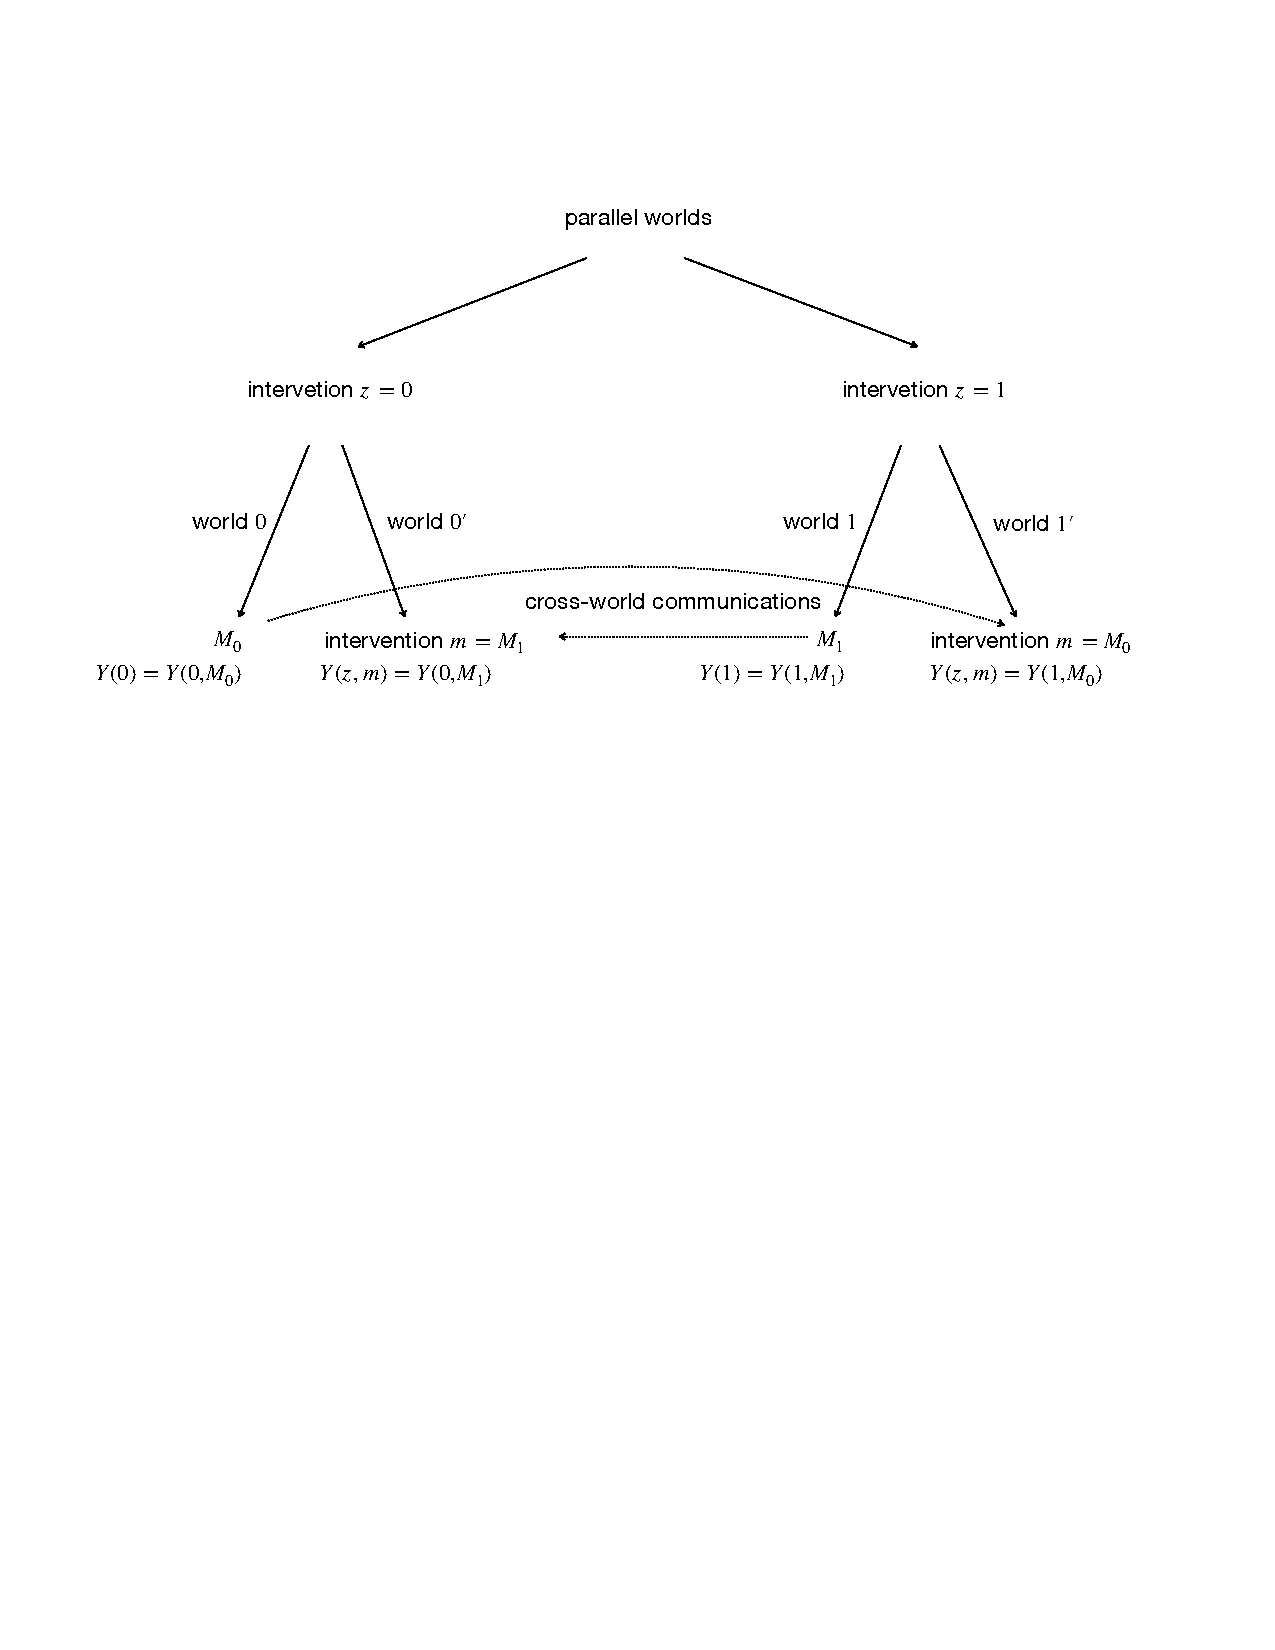
\includegraphics[width =  \textwidth]{figures/crossworld.pdf}
\caption{Cross-world potential outcomes $Y(1,M_0)$ and $Y(0, M_1)$}\label{fg::crossworld}
\end{figure}




\section{The Mediation Formula}

\citet{Pearl::2001}'s mediation formula relies on the following four assumptions. The first three essentially assume that the treatment and the mediator are both randomized conditional on observed covariates.

\begin{assumption}
\label{assume::mediation1}
There is no treatment-outcome confounding: 
$$
Z\ind Y(z,m)\mid X
$$ 
for all $z$ and $m$.
\end{assumption}

\begin{assumption}
\label{assume::mediation2}
There is no mediator-outcome confounding: 
$$
M \ind Y(z,m) \mid (X, Z)
$$ 
for all $z$ and $m$.
\end{assumption}

Assumptions \ref{assume::mediation1} and \ref{assume::mediation2} together are often called {\it sequential ignorability}. They
 are equivalent to the assumption that $(Z, M)$ are jointly randomized conditioning on $X$:
\begin{eqnarray}\label{eq::joint-randomization}
(Z, M) \ind Y(z,m)\mid X
\end{eqnarray} 
for all $z$ and $m$. I leave the proof of \eqref{eq::joint-randomization} as Problem \ref{para::sr-jr}. 



\begin{assumption}
\label{assume::mediation3}
There is no treatment-mediator confounding: 
$$
Z \ind M(z) \mid X
$$ 
for all $z$. 
\end{assumption}

The last assumption is the cross-world independence. 

\begin{assumption}
\label{assume::mediation4}
There is no cross-world independence between the potential outcomes and potential mediators: 
$$
Y(z,m) \ind M(z') \mid X
$$ 
for all $z,z'$ and $m$. 
\end{assumption}


Assumptions \ref{assume::mediation1}--\ref{assume::mediation3} are very strong, but at least they hold under experiments with randomized treatment and mediator. Assumption \ref{assume::mediation4} is stronger because no physical experiment can ensure it. Because we can never observe $Y(z,m)$ and $ M(z') $ in any experiment if $z\neq z'$, Assumption \ref{assume::mediation4}  can never be validated so it is fundamentally metaphysical. 

I give an example below in which Assumptions \ref{assume::mediation1}--\ref{assume::mediation4} all hold. 

\begin{example}
\label{eg::mediation-assumptions}
Given $X$, we generate
\begin{eqnarray*}
Z &=& 1\{  g_Z(X, \varepsilon_Z)  \geq 0 \} ,\\
M(z) &=& 1\{   g_M(X, z, \varepsilon_M)  \geq 0 \} ,\\
Y(z,m) &=& g_Y(X, z, m, \varepsilon_Y ),
\end{eqnarray*}
for $z,m = 0,1$,
where 
$
\varepsilon_Z, \varepsilon_M,
\varepsilon_Y 
$
are all independent random errors. Consequently, we generate the observed values of $M$ and $Y$ from
\begin{eqnarray*}
M &=& M(Z) = 1\{   g_M(X, Z, \varepsilon_M)  \geq 0 \},\\
Y &=& Y(Z,M) = g_Y(X, Z, M, \varepsilon_Y ) . 
\end{eqnarray*}
We can verify that Assumptions \ref{assume::mediation1}--\ref{assume::mediation4}  hold under this data-generating process.
On the contrary, if we allow $  \varepsilon_M$ and $\varepsilon_Y$ to be $ \varepsilon_M(z)$ and $\varepsilon_Y(z,m)$, then Assumptions \ref{assume::mediation1}--\ref{assume::mediation4} can fail. 
See Problem \ref{para::mediation-assumptions-DGP} for more details.
\end{example}



\citet{Pearl::2001} proved the following key result for mediation analysis. 

\begin{theorem}
\label{thm::mediation}
Under Assumptions \ref{assume::mediation1}--\ref{assume::mediation4},  we have 
$$
E\{ Y(z, M_{z'})  \mid X=x \} =  \sum_m E(Y\mid Z=z, M=m, X=x) \pr(M =  m \mid Z=z', X=x)   
$$
and therefore,
\begin{eqnarray*}
&&E\{ Y(z, M_{z'})   \}  \\
&=&  \sum_x E\{ Y(z, M_{z'})  \mid X=x \} \pr(X =  x )  \\
&=&  \sum_x \sum_m E(Y\mid Z=z, M=m, X=x) \pr(M =  m \mid Z=z', X=x)   \pr(X =  x ).
\end{eqnarray*}
\end{theorem}

 

Theorem \ref{thm::mediation} assumes that both $M$ and $X$ are discrete. With general $M$ and $X$, the mediation formulas become
$$
E\{ Y(z, M_{z'}) \mid X=x  \} =   \int  E(Y\mid Z=z, M=m, X=x) f ( m \mid Z=z', X=x) \d m
$$
and
\begin{eqnarray*}
&&E\{ Y(z, M_{z'})   \}  \\
 &=& \int E\{ Y(z, M_{z'}) \mid X=x  \}   f  (x) \d x  \\
 &=& \int \int  E(Y\mid Z=z, M=m, X=x) f ( m \mid Z=z', X=x)     f  (x) \d m \d x   . 
\end{eqnarray*}
From Theorem \ref{thm::mediation}, the identification formulas for the means of the nested potential outcomes depend on the conditional mean of the outcome given the treatment, mediator, and covariates, as well as the conditional mean of the mediator given the treatment and covariates. We need to evaluate these two conditional means at different treatment levels if the nested potential outcome involves cross-world interventions. 

If we drop the cross-world independence assumption, we can modify the definition of the natural direct and indirect effects and the same formulas hold. See Problem \ref{problem::no-crossworld-modification} for more details.  

I give the proof below. 
 

\begin{myproof}{Theorem}{\ref{thm::mediation}}
By the tower property, $E\{ Y(z, M_{z'})   \}  =  E[ E\{ Y(z, M_{z'})  \mid X\}  ]$, so we need only to prove the formula for $E\{ Y(z, M_{z'})  \mid X=x\}$. 
Starting with the law of total probability, we have
\begin{eqnarray*}
&& E\{ Y(z, M_{z'})  \mid X=x\}  \\
&=& 
\sum_m E\{ Y(z, M_{z'})  \mid  M_{z'} = m, X=x\} \pr(  M_{z'} = m\mid X=x) \\
&=&
\sum_m E\{ Y(z, m)  \mid  M_{z'} = m, X=x\} \pr(  M_{z'} = m\mid X=x) \\ 
&=& 
\sum_m \underbrace{ E\{ Y(z, m)  \mid    X=x\} }_{\text{Assumption }\ref{assume::mediation4} } 
\underbrace{ \pr(  M  = m\mid Z=z' , X=x) }_{\text{Assumption }\ref{assume::mediation3} } \\ 
&=&
\sum_m \underbrace{E( Y  \mid  Z=z, M=m,   X=x)}_{ \text{Assumptions }\ref{assume::mediation1}\text{ and }\ref{assume::mediation2} } 
\pr(  M  = m\mid Z=z' , X=x) .
\end{eqnarray*}
%Averaging over $X$, we obtain the mediation formula. 
\end{myproof}


The above proof is trivial from a mathematical perspective. It illustrates the necessity of Assumptions \ref{assume::mediation1}--\ref{assume::mediation4}. 


Conditional on $X=x,$ the mediation formulas for $Y(1, M_1)$ and $Y(0, M_0)$ simplify to
\begin{eqnarray*}
&& E\{  Y(1, M_1)\mid X=x \} \\ 
&=& \sum_m E( Y  \mid  Z=1, M=m,   X=x) \pr(M=m \mid Z=1, X=x)\\
&=& E( Y  \mid  Z=1 ,  X=x)
\end{eqnarray*}
and
\begin{eqnarray*}
&&E\{  Y(0, M_0)\mid X=x \}  \\
&=& \sum_m E( Y  \mid  Z=0, M=m,   X=x) \pr(M=m \mid Z=0, X=x)\\
&=& E( Y  \mid  Z=0 ,  X=x)
\end{eqnarray*}
based on the law of total probability; the mediation formula for $Y(1, M_0)$ simplifies to
\begin{eqnarray*}
&&E\{  Y(1, M_0)\mid X=x \}  \\
&=&  \sum_m E( Y  \mid  Z=1, M=m,   X=x) \pr(M=m \mid Z=0, X=x),
\end{eqnarray*}
where the conditional expectation of the outcome is given $Z=1$ but the conditional distribution of the mediator is given $Z=0$. 
This leads to the identification formulas of the natural direct and indirect effects.

\begin{corollary}
\label{corollary::mediation-nde-nie}
Under Assumptions \ref{assume::mediation1}--\ref{assume::mediation4}, 
the conditional natural direct and indirect effects are identified by
\begin{eqnarray*}
\NDE(x) &=& E\{ Y(1, M_0) - Y(0, M_0) \mid X=x \} \\
&=& \sum_m \{ E( Y  \mid  Z=1, M=m,   X=x) - E( Y  \mid  Z=0, M=m,   X=x) \} \\
&& \qquad  \times \pr(M=m \mid Z=0, X=x)
\end{eqnarray*}
and
\begin{eqnarray*}
\NIE(x) &=& E\{ Y(1, M_1) - Y(1, M_0) \mid X=x \} \\
&=& \sum_m   E( Y  \mid  Z=1, M=m,   X=x)\\
&&  \qquad  \times  \{ \pr(M=m \mid Z=1, X=x) -  \pr(M=m \mid Z=0, X=x) \};
\end{eqnarray*}
the unconditional ones can be identified by $\NDE = \sum_ x \NDE(x) \pr(X=x)$ and $\NIE = \sum_ x \NIE(x) \pr(X=x)$.
\end{corollary}





As a special case, with a binary $M$, the formula of the $\NIE$ reduces to a product form below.


\begin{corollary}
\label{corollary::mediation-binary-M}
Under Assumptions \ref{assume::mediation1}--\ref{assume::mediation4}, for a binary mediator $M$, we have 
$$
\NIE(x)  =      \tau_{Z\rightarrow M} (x) \tau_{M\rightarrow Y} (1,x)
$$
and
$
\NIE = E\{  \NIE(X)   \},
$
where
$$
\tau_{Z\rightarrow M}(x) =  \pr(M=1 \mid Z=1, X=x) -  \pr(M=1 \mid Z=0, X=x) . 
$$
and
$$
\tau_{M\rightarrow Y} (z,x) = E( Y  \mid  Z=z, M=1,   X=x) - E( Y  \mid  Z=z, M=0,   X=x)
$$
\end{corollary}

I leave the proof of Corollary \ref{corollary::mediation-binary-M} as Problem \ref{para::nie-binary-m}. 
Corollary \ref{corollary::mediation-binary-M} gives a simple formula in the case of a binary $M$. 
With randomized $Z$ conditional on $X$, we can view $\tau_{Z\rightarrow M}(x) $ as the conditional average causal effect of $Z$ on $M$. With randomized $M$ conditional on $(X,Z)$, we can view $\tau_{M\rightarrow Y} (z,x) $ as the conditional average causal effect of $M$ on $Y$. The conditional natural indirect effect equals their product. This is coherent with our intuition that the indirect effect acts from $Z$ to $M$ and then from $M$ to $Y$. 


\section{The Mediation Formula Under Linear Models}


Theorem \ref{thm::mediation} gives the nonparametric identification formula for mediation analysis. It allows us to derive various formulas for mediation analysis under different models. I will introduce the famous Baron--Kenny method under linear models below.
\citet{vanderweele2015explanation} gives explicit formulas for the natural direct and indirect effects for many commonly used models. I  relegate the details of other models to Section \ref{chapter::mediation-problmes}. 

\subsection{The Baron--Kenny Method}


\begin{figure}[ht]
\centering
$$
\begin{xy}
\xymatrix{
&  & X \ar[ddll] \ar[dd]^{\beta_2} \ar[ddrr]^{\theta_4} \\
&&\\
Z \ar[rr]^{\beta_1} \ar@/_2.8pc/[rrrr]_{\theta_1} & & M\ar[rr]^{\theta_2} & & Y & \text{indirect effect: } \beta_1\theta_2 \\
&&&&& \text{  direct effect: } \theta_1 }
\end{xy}
$$
\caption{The Baron--Kenny method for mediation under linear models}\label{fg::mediationDAG-BK}
\end{figure}

The Baron--Kenny method assumes the following linear models for the mediator and outcome given the treatment and covariates.

\begin{assumption}
[linear models for the Baron--Kenny method]
\label{assume::mediation-bk-model}
Both the mediator and outcome follow linear models:
$$
\left\{\begin{array}{rcl}
E(M \mid Z, X) &=&  \beta_0 + \beta_1 Z + \beta_2\tran X, \\
E(Y\mid Z,M,X) &=& \theta_0 + \theta_1 Z + \theta_2 M + \theta_4\tran X.
\end{array}\right.
$$
\end{assumption}


 
Under these linear models,  the formulas for the natural direct and indirect effects simplify to functions of the coefficients. 

\begin{corollary}
[Baron--Kenny formulas for mediation]
\label{corollary::bk-formulas}
Under Assumptions \ref{assume::mediation1}--\ref{assume::mediation4} and \ref{assume::mediation-bk-model},  we have 
$$
\NDE = \theta_1
,\quad 
\NIE = \theta_2 \beta_1 .
$$
\end{corollary}


The formulas in Corollary \ref{corollary::bk-formulas} are intuitive based on Figure \ref{fg::mediationDAG-BK}. The direct effect equals the coefficient on the path $Z\rightarrow Y$, and the indirect effect equals the product of the coefficients on the path $Z\rightarrow M\rightarrow Y$. I give the proof below based on Theorem \ref{thm::mediation}. 


\begin{myproof}{Corollary}{\ref{corollary::bk-formulas}}
The conditional NDE equals 
$$
\NDE(x)  
= \sum_m  \theta_1  \pr(M=m \mid Z=0, X=x) = \theta_1
$$
and the conditional NIE equals 
\begin{eqnarray*}
\NIE(x) &=&  \sum_m  (\theta_0 + \theta_1  + \theta_2 m + \theta_4\tran x )\\
&&  \qquad  \times  \{ \pr(M=m \mid Z=1, X=x) -  \pr(M=m \mid Z=0, X=x) \} \\
&=& \theta_2 \{ E(M=m \mid Z=1, X=x) -  E(M=m \mid Z=0, X=x) \} \\
&=&  \theta_2 \beta_1 ,
\end{eqnarray*}
which do not depend on $x$. Therefore, they are also the formulas for the unconditional natural direct and indirect effects.
\end{myproof}


 
If we obtain OLS estimators of these coefficients, we can estimate the direct and indirect effects by
$$
\hat{\NDE} = \hat{\theta}_1,\qquad
\hat{\NIE} = \hat{\theta}_2 \hat{\beta}_1,
$$
which is called the Baron--Kenny method \citep{Judd::1981, baron1986moderator} although it had several antecedents \citep[e.g.,][]{hyman1955survey, alwin1975decomposition, Judd::1981, sobel1982asymptotic}.


Standard software packages report the standard error of $\hat{\NDE}$ from OLS. \citet{sobel1982asymptotic, sobel1986some} used the delta method to obtain the standard error of $\hat{\NIE}$. 
%Based on the heuristics:
%\begin{eqnarray*}
%\hat{\theta}_2  \hat{\beta}_1 -  \theta_2 \beta_1
%&=& \hat{\theta}_2  \hat{\beta}_1 -  \theta_2 \hat{\beta}_1 +   \theta_2 \hat{\beta}_1  -  \theta_2 \beta_1 \\
%&=&  (\hat{\theta}_2 -  \theta_2 )  \hat{\beta}_1 + \theta_2 (\hat{\beta}_1 - \beta_1 ) \\
%&\approx& (\hat{\theta}_2 -  \theta_2 )   \beta_1 + \theta_2 (\hat{\beta}_1 - \beta_1 )
%\end{eqnarray*}
%and the independence of $\hat{\theta}_2 $ and $ \hat{\beta}_1$, 
Based on the formula in Example \ref{example::asymptotic-normal-product},  the asymptotic variance of $\hat{\theta}_2  \hat{\beta}_1 $ equals 
$
\var(\hat{\theta}_2)  \beta_1^2 + \theta_2^2 \var(\hat{\beta}_1) .
$
So the estimated variance is
$$
\hat{\var}(\hat{\theta}_2)  \hat{\beta}_1^2 + \hat{\theta}_2^2 \hat{\var}(\hat{\beta}_1) .
$$
Testing the null hypothesis of $\NIE$ based on $\hat{\theta}_2 \hat{\beta}_1$ and the estimated variance above is called {\it Sobel's test} in the literature of mediation analysis. 


 


\subsection{An Example}\label{section::BK-jobs}

We can easily implement the Baron--Kenny method via the following code. 

 \begin{lstlisting}
library("car")
BKmediation = function(Z, M, Y, X)
{
  ## two regressions and coefficients
  mediator.reg   = lm(M ~ Z + X)
  mediator.Zcoef = mediator.reg$coef[2]
  mediator.Zse   = sqrt(hccm(mediator.reg)[2, 2])
  
  outcome.reg    = lm(Y ~ Z + M + X)
  outcome.Zcoef  = outcome.reg$coef[2]
  outcome.Zse    = sqrt(hccm(outcome.reg)[2, 2])
  outcome.Mcoef  = outcome.reg$coef[3]
  outcome.Mse    = sqrt(hccm(outcome.reg)[3, 3])
  
  ## Baron-Kenny point estimates
  NDE = outcome.Zcoef
  NIE = outcome.Mcoef*mediator.Zcoef
  
  ## Sobel's variance estimate based the delta method
  NDE.se = outcome.Zse
  NIE.se = sqrt(outcome.Mse^2*mediator.Zcoef^2 + 
                  outcome.Mcoef^2*mediator.Zse^2)
  
  res = matrix(c(NDE, NIE, 
                 NDE.se, NIE.se,
                 NDE/NDE.se, NIE/NIE.se), 
               2, 3)
  rownames(res) = c("NDE", "NIE")
  colnames(res) = c("est", "se", "t")
  
  res
}
 \end{lstlisting}
 
 
 Revisiting Example  \ref{eg::mediation-jobs}, we obtain the following estimates for the direct and indirect effects:
 
 \begin{lstlisting}
> jobsdata = read.csv("jobsdata.csv")
> Z = jobsdata$treat
> M = jobsdata$job_seek
> Y = jobsdata$depress2
> getX     = lm(treat ~ econ_hard + depress1 + 
+                 sex + age + occp + marital + 
+                 nonwhite + educ + income,
+               data = jobsdata)
> X = model.matrix(getX)[, -1]
> res = BKmediation(Z, M, Y, X)
> round(res, 3)
       est    se      t
NDE -0.037 0.042 -0.885
NIE -0.014 0.009 -1.528
\end{lstlisting}

Both the estimates for the direct and indirect effects are negative although they are insignificant. 



\section{Sensitivity analysis}


Mediation analysis relies on strong and untestable assumptions. One crucial assumption is that there is no unmeasured confounding among the treatment, mediator, and outcome. Various sensitivity analysis methods appeared in the literature. In particular, \citet{ding2016sharp} proposed Cornfield-type sensitivity bounds, and \citet{zhang2022interpretable} proposed a sensitivity analysis method tailored to the Baron--Kenny method based on linear structural equation models. These are beyond the scope of this book.  





 

\section{Homework problems}\label{chapter::mediation-problmes}



\paragraph{\citet{Robins::1992}'s clarification of the units based on nested potential outcomes}\label{hw::robins1992-latentgroups}


Assume $(Z, M, Y)$ are all binary. Based on the joint value of 
$$
M(1), M(0),  Y(1, M_1), Y(1, M_0), Y(0, M_1), Y(0, M_0) ,
$$
how many types of units do we have?

If we assume monotonicity of $Z$ on $M$, that is,
$$
M(1) \geq  M(0),
$$
then how many types of units do we have?

If we further assume monotonicity of $Z$ and $M$ on $Y$, that is,
$$
Y(1, m) \geq Y(0, m),  \quad Y(z, 1) \geq Y(z, 0)
$$
for all $z$ and $m$, then how many types of units do we have?


\paragraph{Sequential randomization and joint randomization}\label{para::sr-jr}

Show \eqref{eq::joint-randomization} is equivalent to Assumptions \ref{assume::mediation1} and \ref{assume::mediation2}. 


\paragraph{Verifying the assumptions for mediation analysis}\label{para::mediation-assumptions-DGP}

Show that Assumptions \ref{assume::mediation1}--\ref{assume::mediation4} hold under the data generating process in Example \ref{eg::mediation-assumptions}. 
Also show that if we allow $  \varepsilon_M$ and $\varepsilon_Y$ to be $ \varepsilon_M(z)$ and $\varepsilon_Y(z,m)$, then Assumptions \ref{assume::mediation1}--\ref{assume::mediation4} can fail. 
 
 \paragraph{Another set of assumptions for the mediation formula}\label{para::alternative-si}



\citet{Imai::2010} invoked the following set of assumptions to derive the mediation formula. 

\begin{assumption}
\label{assume::mediation-imai}
We have 
$$
\{Y(z, m), M(z') \} \ind  Z\mid X
$$
and
$$
Y(z, m) \ind M(z' ) \mid (Z=z' , X)
$$
for all $z, z', m$.
\end{assumption}


\begin{theorem}
\label{thm::mediation-imai}
Under Assumption \ref{assume::mediation-imai}, the mediation formula in Theorem \ref{thm::mediation} holds. 
\end{theorem}


Prove Theorem \ref{thm::mediation-imai}. 



\paragraph{Difference method and product method are identical}\label{hw::difference=product}


In the main text, we first obtain the OLS fits
$$
\left\{\begin{array}{rcl}
\hat M_i &=&  \hat\beta_0 + \hat\beta_1 Z_i + \hat\beta_2\tran X_i, \\
\hat Y_i &=&\hat \theta_0 + \hat\theta_1 Z_i +\hat \theta_2 M_i + \hat\theta_4\tran X_i.
\end{array}\right.
$$
The estimate for the NIE is the product $\hat \theta_2 \hat\beta_1 $, which is called the product method. 

Alternatively, we can first obtain OLS fits:
$$
\left\{\begin{array}{rcl}
\hat Y_i &=&  \hat\alpha_0 + \hat\alpha_1 Z_i + \hat\alpha_1 \tran X_i, \\
\hat Y_i &=&\hat \theta_0 + \hat\theta_1 Z_i +\hat \theta_2 M_i + \hat\theta_4\tran X_i.
\end{array}\right.
$$
Another estimate for the NIE is the difference $\hat\alpha_1 -  \hat\theta_1$, which is called the difference method. 

Show that $\hat\alpha_1 -  \hat\theta_1 = \hat \theta_2 \hat\beta_1 .$


Remark: Recall Cochran's formula in Problem \ref{hw::cochran+ovb}. 



\paragraph{Natural indirect effect with a binary mediator}\label{para::nie-binary-m}

Prove Corollary \ref{corollary::mediation-binary-M}. 


\paragraph{With treatment-outcome interaction on the outcome}\label{para::interaction}
\citet{vanderweele2015explanation} suggested using the following linear models:
$$
\left\{\begin{array}{rcl}
E(M \mid Z, X) &=&  \beta_0 + \beta_1 Z + \beta_2\tran X, \\
E(Y\mid Z,M,X) &=& \theta_0 + \theta_1 Z + \theta_2 M + \theta_3 ZM + \theta_4\tran X,
\end{array}\right.
$$
where the outcome model has the interaction term between the treatment and the mediator. 


Under the above linear models,  show that 
$$
\NDE = \theta_1 + \theta_3\{ \beta_0 + \beta_2\tran E(X)\}, \qquad 
\NIE = (\theta_2 + \theta_3 ) \beta_1. 
$$
How do we estimate $\NDE$ and $\NIE$ with IID data?

Remark:
Consider the simple case with a binary $Z$ and binary $M$.
Under the linear models, the average causal effect of $Z$ of $M$ equals $\beta_1$, and the average causal effect of $M$ on $Y$ equals $\theta_2 + \theta_3 E(Z)$. Therefore, it is possible that both of these effects are positive, but the natural indirect effect is negative. For instance:
$$
\beta_1 = 1,\quad \theta_2 = 1, \quad  \theta_3= -1.5, \quad E(Z) = 0.5.
$$ 
This is somewhat paradoxical and can be called the {\it mediator paradox}. \citet{chen2007criteria} reported a related {\it surrogate endpoint paradox} or {\it intermediate variable paradox}.



\paragraph{Mediation analysis with continuous mediator and binary outcome}\label{para::continM-binaryY}


Consider the following Normal linear model for the mediator and logistic model for the binary outcome:
$$
\left\{\begin{array}{rcl}
M \mid Z, X &\sim &  \textsc{N}(\beta_0 + \beta_1 Z + \beta_2\tran X, \sigma_M^2), \\
\logit \{ \pr(Y = 1 \mid Z,M,X ) \} &=& \theta_0 + \theta_1 Z + \theta_2 M +   \theta_4\tran X,
\end{array}\right.
$$
where $\logit (w)  = \log\{ w/(1-w) \} $ with inverse $\expit(w) = (1 + e^{-w})^{-1}.$
Express $\NDE$ and $\NIE$ in terms of the model parameters and the distribution of $X$. How do we estimate $\NDE$ and $\NIE$ with IID data?




\paragraph{Mediation analysis with binary mediator and continuous outcome}\label{para::logit-binary-m}
Consider the following logistic model for the binary mediator and linear model for the outcome:
$$
\left\{\begin{array}{rcl}
\logit\{ \pr(M  = 1\mid Z, X) \}&=&  \beta_0 + \beta_1 Z + \beta_2\tran X, \\
E(Y\mid Z,M,X) &=& \theta_0 + \theta_1 Z + \theta_2 M +   \theta_4\tran X . 
\end{array}\right.
$$
%where $\logit (w)  = \log\{ w/(1-w) \} $ with inverse $\expit(w) = (1 + e^{-w})^{-1}.$


Under these models, show that 
$$
\NDE = \theta_1  ,\qquad
\NIE = \theta_2 E \left\{  \expit(\beta_0 + \beta_1  + \beta_2\tran X)
-  \expit(\beta_0   + \beta_2\tran X)  \right\}. 
$$
How do we estimate $\NDE$ and $\NIE$ with IID data?






\paragraph{Mediation analysis with binary mediator and outcome}
\label{para::mediation-binaryMY}

Consider the following logistic models for the binary mediator and outcome:
$$
\left\{\begin{array}{rcl}
\logit\{ \pr(M  = 1\mid Z, X) \}&=&  \beta_0 + \beta_1 Z + \beta_2\tran X, \\
\logit \{ \pr(Y = 1 \mid Z,M,X ) \} &=& \theta_0 + \theta_1 Z + \theta_2 M +   \theta_4\tran X.
\end{array}\right.
$$
Express $\NDE$ and $\NIE$ in terms of the model parameters and the distribution of $X$. How do we estimate $\NDE$ and $\NIE$ with IID data?



  
\paragraph{Modify the definitions to drop the cross-world independence}\label{problem::no-crossworld-modification}


Define 
$$
Y(z, F_{M_{z'}\mid X}) = \int Y(z,m) f(M_{z'} = m\mid X) \d m
$$
as the potential outcome under treatment $z$ and a random draw from the distribution of $M_{z'}\mid X$. 
With a discrete $M$, the definition simplifies to
$$
Y(z, F_{M_{z'}\mid X}) =\sum_m Y(z,m) \pr(M_{z'} = m\mid X).
$$
The key difference between $Y(z,M_{z'})$ and $Y(z, F_{M_{z'}\mid X}) $ is that $M_{z'}$ is the potential mediator for the same unit whereas $F_{M_{z'}\mid X}$ is a random draw from the conditional distribution of the potential mediator in the whole population. 
Define the natural direct and indirect effects as
$$
\NDE = E\{Y(1, F_{M_{0}\mid X})  - Y(0, F_{M_{0}\mid X})   \},\quad
\NIE  =  E\{Y(1, F_{M_{1}\mid X})  - Y(1, F_{M_{0}\mid X})   \}.
$$


Show that under Assumptions \ref{assume::mediation1}--\ref{assume::mediation3}, the identification formulas for $\NDE$ and $\NIE$ remain the same as in the main text. 



Remark: Modifying the definitions of the nested potential outcomes allows us to relax the strong cross-world independence assumption but weakens the interpretation of the natural direct and indirect effects. See \citet{vanderweele2015explanation} for more discussion and \citet{vanderweele2017mediation} for an application to a more complex setting with time-varying treatment and mediator.

  
  
\paragraph{Connections between principal stratification and mediation analysis}

\citet{vanderweele2008simple} and
\citet{forastiere2018principal} reviewed and compared principal stratification and mediation analysis. 
